\documentclass[../main/thesis]{subfiles}

% Overleaf graphics path
\graphicspath{{thesis/discussion/figures/}}

% \graphicspath{{/home/arefk/uio/MScThesis_AreKvanum2022_SeaIceML/thesis/discussion/figures/}}
\begin{document}
\section{Discussion}
\label{sec:discussion}
The following section will discuss the results presented in sections \ref{sec:developing a unet}, \ref{sec:model-perf} and \ref{sec:physical-connections}. The results will be discussed separately and in conjunction where appropriate.

\subsection{Development}
The development of the Deep learning system was described in Section \ref{sec:developing a unet}, and encompasses data preparation, architectural considerations as well as hyperparameter tuning. The overall goal for the model development is to find the optimal combination of predictor configurations and model implementation which results in a Deep learning system with low error and high generalizability (Section \ref{sec:training-loop}).

\subsubsection{Initial attempt}
\label{sec:multiclass-intitial}
Section \ref{sec:singleoutputmodel} presents the initial attempt at designing a deep learning architecture for sea ice category classification. The initial architecture closely resembled the U-Net architecture as described by \citet{Ronneberger2015}, and contains a single output layer with multiple channels such that multiple classes are predicted at the same time. This follows the U-Net architecture and training procedure descriptions given in sections \ref{sec:unet} and \ref{sec:training-loop}, where each channel in the output layer is representing a target class in contrast to the cumulative contour approach described in Section \ref{sec:data_targets}. Each channel in the output contains unactivated probabilities (logits) for each pixel to belong to the class. To determine which category each pixel is most likely to belong to, the softmax function (Equation \ref{eq:psoftmax}) converts the logits to probabilities where each pixel is assigned the category belonging to the channel with highest probability. As seen in figure \ref{fig:singleoutmodel}, neither the $(40 - 60\%)$ nor $(70 - 80\%)$ categories are resolved. This result (not shown) occurs for all samples in the 2022 test data. It appeared from the monthly distribution of sea ice categories presented in figure \ref{fig:2022-areadist-sic} that the intermediate sea ice categories (very open drift ice, open drift ice, close drift ice) constituted a significantly low fraction of the different sea ice categories. Due to the skewness in the sea ice category distribution towards ice free open water and very close drift seen in the sea ice charts, the current formulation of the segmentation task is highly imbalanced in favour of the aforementioned classes. Furthermore, due to the presence of class imbalance, it is expected that the computed loss (which is the unweighted variant of Equation \ref{eq:unet-loss}) is dominated by the more likely classes. Assuming that each contribution to the loss is treated equally due to the absence of a class- or pixel level weight term, the more likely classes supply a larger fraction of the learning signal. This is shown in \citet{Lin2017} and has the potential to dwarf or counteract the portion of the learning signal computed from the less likely classes.

With regards to the intended operationality and usefulness of the developed deep learning system, resolving the MIZ is a crucial aspect to achieve skillful forecasts that ensure maritime safety \citep{Wagner2020}. Considering the above discussion, it is likely that the model is not predicting the intermediate MIZ classes due to the model-training consistently computing a loss in favour of the more likely (not intermediate) classes, which is further reinforced every epoch as a consequence of the class-imbalance (figure \ref{fig:2022-areadist-sic}). One way to approach the problem of class imbalance would be to modify the weight parameter $w$ in equation \ref{eq:unet-loss}. In the work of \citet{Ronneberger2015}, $w$ was defined as a precomputed weight map which assigned some pixels more importance than others to compensate for the different frequency of pixels between the classes. However, it is noted that the weight map computed by \citet{Ronneberger2015} is specifically designed for biomedical image segmentation, and not directly transferable to other domains. Another approach which indirectly defines the weight $w$ is through rewriting the loss function, such as the focal loss proposed by \citet{Lin2017}. The focal loss introduces a focusing parameter and a modulating factor which down-weights the loss contribution from predictions with a high probability, i.e. easy to predict samples contribute less to the total loss \citep{Lin2017}. Another way to approach the problem of class imbalance is to reformulate the prediction task to a more balanced problem as described in section \ref{sec:data_targets} with the introduction of cumulative contours. Due to the immediate improvement in contour resolve seen when implementing the cumulative contours, the approach was further pursued in favour of the single output layer model.

\subsubsection{Determining the depth of the model}
\label{sec:discuss_depth}
Finding the optimal learning rate and depth of the desired deep learning architecture (multiple outputs, single label) is summarized in figures \ref{fig:gs} and \ref{fig:loss_curve_from_gs}. Based on the conducted grid search in figure \ref{fig:gs}, we see that the validation loss tends to increase when the model becomes deeper, as well as when deviating from $lr = 0.001$. Although the lowest validation loss is achieved with $lr = 0.001$ and a depth of 512 channels in the bottleneck, the difference is marginal compared to the 256 depth counterpart. However, the model with a depth of 256 channels has 4 times less parameters than the 512 depth model, which indicates that the 256 model is satisfactory fit to the data without needing the additional parameters found in the deeper network. This is further indicated by figure \ref{fig:loss_curve_from_gs}, which shows that the 256-depth model is marginally improved beyond the 10th epoch. 

When comparing a prediction from a 1024 depth U-Net with a 256 depth U-Net (figure \ref{fig:256_1024_compare}), the predictions are generally visually similar. The similarity can be further seen when comparing the difference in NIIEE, which is 2.5km (a difference of 8\%) less for the 256 depth U-Net. As such, the increased complexity gained from increasing the parameter-count of the model does not seem necessary to increase the predictive skill of the model. Viewed in conjunction with figure \ref{fig:loss_curve_from_gs}, a possible explanation may be that the 256 model already rapidly fits the training data. Hence, a more complex architecture in terms of encoder depth is not needed.

Using Equation \ref{eq:receptivefield}, which was derived from \citet{Araujo2019}, it was calculated that the bottleneck of the 256 encoder have a theoretical receptive field of 145 pixels in each direction, whereas the 1024 encoder have a receptive field covering the entirety of the input fields. As such, each high level feature in the 256 bottleneck has only been influenced by lower level features in a 145km radius, whereas each high level feature in the bottleneck of the 1024 model has been influenced by features from the entirety of the input domain. Although the encoded signals in the 1024 bottleneck contain influences from the entire input field, figure \ref{fig:gs} and \ref{fig:256_1024_compare} indicate that the performance is still reduced, as the model has a higher NIIEE compared to the 256 model with a limited influential range for the bottleneck. 

It is shown in \citet{Luo2017} that the effective receptive field is limited compared to the theoretical receptive field, with the effective receptive field attaining an asymptotic gaussian shape. \citet{Luo2017} also show an example where although the theoretical receptive field is bigger than the input size, the effective receptive field is not able to fit the whole image, which is a consequence of the relative shrink of the effective receptive field shown to follow the relationship $\propto \frac{1}{\sqrt{N}}$ where N is the number of layers \citep{Luo2017}. Thus, based on the results of \citet{Luo2017}, all features of the bottleneck in the 1024 depth U-Net are unlikely to be influenced by the entirety of the input domain despite the coverage implied by the theoretical receptive field. On the contrary, the result of \citet{Luo2017} suggests that predictor resolution determine the influential radius of which feature maps are able to capture spatial dependencies from, more so than the U-Net architecture. Since the effective receptive field causes high level features to be influenced mostly by the locally surrounding pixels, the resolution of the predictors determine the spatial extent of the local neighborhood. Thus if the predictors are high-resolution, the higher level feature maps will mostly be influenced by local physical processes.

Moreover, to attain a theoretical receptive field which covered the full input domain, the model complexity had to be increased by a factor of $\sim 16$. Thus, the current results seems to discourage the need of fitting deep and complex neural networks to high resolution and spatially dependent data, since their theoretical ability to encode high level features influenced by all grid cells from the input data is opposed by a combination of the increased model complexity and reduced effective receptive field fraction influenced by the resolution of the predictors.

\subsubsection{Demonstrating seasonality}
\label{sec:demonstrate_seasonality}
The deep learning system is able to preserve seasonality, as indicated by figure \ref{fig:timeseries} which show that the predicted sea ice concentration for a 2 day lead time follows the observed sea ice edge for all months. Based on the demonstrated predictive capabilities of the model seen in Figure \ref{fig:timeseries}, it can be seen that the Deep learning system is able to recreate the seasonal variability of the sea ice edge. Furthermore, the Deep learning model is able to follow the seasonal cycle of sea ice concentration from the input predictors only, which as shown in Figure \ref{fig:data_pipeline} are all two dimensional fields containing a physical quantity. This indicates that the model is able to infer the day of year based on the combined state of the sea ice concentration and atmosphere, which contrasts the work of \citet{Grigoryev2022}, where the date was explicitly given to the model as a predictor. Thus, the model is able to capture the seasonal differences of sea ice dynamics from physical input fields only.

\subsubsection{Using NIIEE as a metric}
Throughout this thesis, model performance have been measured according to the normalized sea ice edge displacement error \citep{Goessling2016, Melsom2019, Palerme2019, Zampieri2019} for different contours. The works of \citet{Goessling2016, Palerme2019, Zampieri2019} all apply the IIEE (or the Spatial Probability Score \citep{Goessling2018}, which is a probabilistic variation of the IIEE) to seasonal prediction systems with coarse spatial resolution ($\gg1$km). Given that the IIEE is proportional to the number- and size of the grid cells, it is explored how the IIEE responds when used in a high spatial resolution sea ice concentration context. Moreover, the validity of deriving the NIIEE from a high resolution IIEE with a coarser resolution sea ice edge length is also inspected in section \ref{sec:clim_iceedge_compute}. Firstly, based on the correlations between the NIIEE computed from both SIC and sea ice edge at 1km and NIIEE where both fields were at 10km resolution, the NIIEE is invariant to the choice of resolution and preserved when used in 1km resolution environments.

Secondly, when dividing the IIEE from a 1km spatial resolution grid by a sea ice edge length computed from a 10km sea ice concentration field, the variability of the NIIEE is similar as when the 1km IIEE is divided by a 1km sea ice edge length (figure \ref{fig:iiee_1km_10km}). The results indicate that the IIEE is a relevant metric also when applied to high spatial resolutions. Moreover, the variability of the NIIEE is preserved with increasing sea ice edge resolutions. Note that the sea ice edges used in section \ref{sec:clim_iceedge_compute} were not independent of the sea ice concentration, which is the case with the sea ice edge length derived from OSI SAF CDR.

With regards to model selection, it was shown in section \ref{sec:connecting_val_loss_with_NIIEE} and figure \ref{fig:val_loss_iiee} that the correlation between the NIIEE and validation loss is strong with a value of 0.82. Moreover, figure \ref{fig:val_loss_iiee} presents an example training where after each epoch, the model was measured in terms of the NIIEE on the validation set. As validating the deep learning system against the NIIEE was considerably slower (2 hours) compared to validating against the validation loss (8 minutes) for a single epoch, it was decided to select models in terms of the validation loss since the correlation between the metrics is strong.

\subsubsection{Increasing the size of the training data}
\label{sec:increase_data}
The size of the core training data (2019 and 2020) of 390, 289 or 286 samples for 1, 2 and 3 day lead time respectively is considerably small when training an encoder-decoder deep learning model. Furthermore, the strong autocorrelation seen in the sea ice charts (figure \ref{fig:autocorr}) may act to further homogenize the total training dataset, as the sea ice concentration for consecutive days have a low variability which may cause samples which are close in time to have a similar latest sea ice chart predictor \citep{Fritzner2020}. However, by increasing the predictor pool through introducing atmospheric variables from AROME Arctic, the deep learning model is also learning correlations between the sea ice concentration development and atmospheric (temperature and wind fields) development. Hence, the strong autocorrelation seen in the sea ice concentration (figure \ref{fig:autocorr}) may not cause the unwanted effect of rendering certain samples redundant, as the atmospheric predictors allows the model to learn a more complex pattern from the input data.

It was mentioned in section \ref{sec:dataloader} that the core training data only consists of the year 2019 and 2020 due to a major update regarding the representation of near surface temperature. It is common to assume that all data used to train, test and validate a machine learning algorithm is Independently and Identically Distributed (IID), but this assumption does not hold when using predictors from AROME Arctic which has been continuously updated after it was released \citep{Mueller2017}. The choice of limiting the training dataset to the aforementioned two year period was made based on an assessment of which updates would have a strong influence on the IID assumption for the chosen variables, where the snow on ice parameterization was deemed particularly significant \citep{Batrak2019}. An example of how the updated changed the near surface temperature distribution can be seen in figure \ref{fig:aa-history}, where a clear bias reduction compared to observations occurs following the update.

\begin{figure}
    \centering
    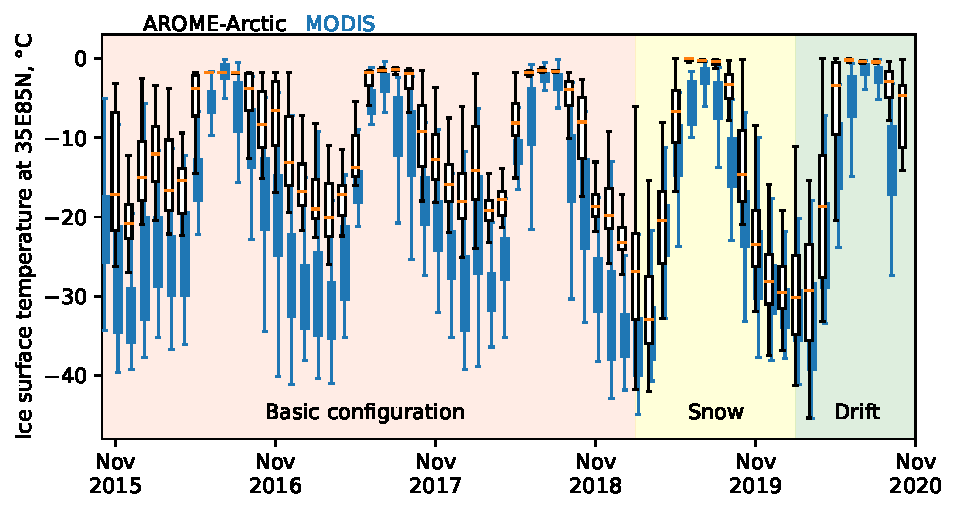
\includegraphics[width=.9\textwidth]{aa-history}
    \caption{\label{fig:aa-history}Ice surface temperature from AROME-Arctic compared with observations. Arome Arctic is distributed as white boxes, whereas observations are blue boxes. The snow on ice parameterization was added starting at the yellow background. Figure courtesy of Yurii Batrak.}
\end{figure}

However, with regards to the problems occurring as a consequence of limited data, the effect of training on an increasing amount of years was shown in figure \ref{fig:append_years}. From figure \ref{fig:append_years}, it can be seen that both the NIIEE and validation loss is reduced when 2017 and 2018 is prepended to the training dataset, although 2016 causes the model to lose skill. Figure \ref{fig:NIIEE-and-SIE} shows that the sea ice charts for the years covered by the training, validation and test dataset follow a similar distribution. Furthermore, there are no trends or clear outlier between the years. As such, it can be assumed that the sea ice charts are IID also when the training data has additional years prepended. Thus, the loss of skill caused by 2016 is likely to be caused by predictors from AROME Arctic which, due to continuous model development, are not IID. That the loss of skill only happens with 2016 included could be a reflection of 2016 being the first full year of operation for AROME Arctic, and it is expected that significant updates occurred frequently during AROME Arctics' first year of operation.

It should also be noted that the inclusion of 2017 and 2018 seems to improve model performance, despite the years not including the snow on ice parameterization deemed significant with regards to the representation of t2m. This could be explained by the model being more impacted by the winds rather than the temperature from AROME Arctic, thus causing the shift in temperature variance to be negligible. A further discussion of predictor importance and model explainability will be done in Section \ref{sec:discuss_explain}.

Figure \ref{fig:append_years} highlights the difficulties of fitting a deep learning model to data from an operational product, as the data are updated frequently in order to improve the product performance through intentional shifts in model bias or variance \citep{Batrak2019} (see also figure \ref{fig:aa-history}). This highlights that there are fundamental conflicting interests in terms of dataset consistency for operational numerical weather prediction output data and data used to train a deep learning network.

It was mentioned in section \ref{sec:arome} that reanalysis products such as CARRA \citep{Koeltzow2022} or ERA5 \citep{Hersbach2020} would alleviate the problem of temporal inconsistencies in the data, as the model used to create a reanalysis is based on a single model cycle. However, reanalysis products generally have a publishing delay from days to months, which is not compatible with the operational timeliness of providing forecasts on the same day as the predictors are valid as  intended for the developed Deep learning system. Furthermore, a reanalysis differs from a forecast in that data is complete and consistent, which in terms of the temporal mean approach for the atmospheric predictors would limit the data diversity as the reanalysis would provide the same values for a given date regardless of the initialization date of the deep learning forecast. This is contrasted by a forecast, which output different values at shared timestamps depending on the forecast initialization date. Hence, despite the expected increase in skill of a reanalysis product due to consistency in the data, the above may serve to limit the overall usefulness for reanalysis products as deep learning predictors in the case where there is a temporal overlap between predictors. 

Although this project has attempted to increase the dataset size directly by adding more data, similar studies utilized other techniques such as \citet{Grigoryev2022} which trained their deep learning model on multiple regions and performed geometric transformations on the data during training. Their results show that geometric augmentations have a small positive influence for some areas, and negligible for one area. Though adding multiple regions to increase dataset size is outside the boundaries of this work, applying geometric augmentations to the data is a known generalization technique for image based deep learning which \citet{Grigoryev2022} could alleviate the limited dataset if implemented correctly \citep{Shorten2019}. However, given that atmospheric variables have a strong spatial dependency inferred by their lat/lon coordinates, it is questioned to what extent geometric transformations applied to the entirety of a scene can teach the network new relations between the variables.

\subsubsection{Exploring model response to land representation}
\label{sec:tuning_model}
The effect of interpolating sea ice concentration over land covered pixels following the approach of \citet{Wang2017} was described in section \ref{sec:modifyhyperparam}. The approach was compared with assigning all land-covered pixels as the category ice free open water (open-ocean mask), where the latter approached increased the mean annual NIIEE with 1.5km. This shows that since all input predictors need have values for all pixels \citep{Ronneberger2015}, how the sea ice is represented in areas which are covered by land impacts how surrounding grid cells are classified. Moreover, the results show that supplying the land-sea mask as a predictor is by itself not sufficient to teach the network to discern between land pixels and water pixels, which may be explained by how the convolutional kernel computes features from a local neighborhood separately for each channel \citep{Fukushima1980}.

Another interpretation of the open-ocean mask is that it relates the affected predictor to be treated as an incomplete partial convolution \citep{Liu2018}. Partial convolution is a variation of the convolutional layer which stem from image inpainting, which is the task of filling holes in an image \citep{Liu2018}. The technique involves multiplying the convolutional filter with a masked variation of the local neighborhood determined by the holes in the image, then the computed value is scaled to adjust for the number of unmasked pixels in the neighborhood \citep{Liu2018}. Since the integration of the land-sea mask into a predictor through the open-ocean mask was without a consideration of scaling the output with regards to the varying number of masked pixels in the local neighborhood, the sharp gradient computed between land-fast ice and ice-free open water is left unscaled thus detected as a notable feature. Thus, the work of \citet{Liu2018} may provide a possible explanation as to why the open ocean mask degrades the performance of the model. 

However, the work of \cite{Liu2018} also highlights a different approach to integrate the land-sea mask into the predictors, as partial convolutions would make it possible to mask a subset or all predictors with the land sea mask thus removing it from the pool of predictors. This may aid to increase the relevance of the land-sea mask, as although the intended behavior of the predictor was to help the model treat land pixels differently than oceanic pixels, it was previously discussed that this behavior was not directly inferred from the land-sea mask. By utilizing partial convolutions, and using the land-sea mask as a mask, the result from convolution would depend only on the oceanic grid points \citep{Liu2018}.

\subsubsection{Tuning model architecture}
Reducing the number of classes to output does not seem to improve the model performance. The model trained in section \ref{sec:modifyhyperparam} where the $> 0\%$ and $=100\%$ contours was removed performs similarly to the Deep learning system which outputs all target classes, with an increase of the NIIEE of 0.4km. This result may suggest that although removing contours have a theoretical impact on training, the effect is not reflected by the predictions. From the description of how the individual losses computed with equation \ref{eq:loss} are treated as a sum starting at the decoder during backpropagation (section \ref{sec:train_env}), it can be seen that removing contours decreases the magnitude of the loss function. Moreover, due to the cumulative contours formulation, removing outputs also has the effect of lowering the amount of redundant information since the number of overlapping pixels are reduced. Hence, the result of removing contours, especially the $100\%$ contour, is that the computed loss is less weighted by the land-fast ice pixels common in all cumulative contours.

The mean seasonal confidence fields from figure \ref{fig:confidence_seasonal} can be used in conjunction with the loss function defined in equation \ref{eq:loss} to determine the impact of the $=100\%$ contour on the overall loss starting from the decoder. Equation \ref{eq:loss} is defined such that a greater deviation from the true value (1) results in a greater loss. Moreover, the $=100\%$ contour is usually present beneath the land areas as the fast-ice contour drawn close to land by the sea ice specialist is interpolated onto the land-pixels by the nearest neighbor interpolation \citep{Wang2017} performed on the sea ice charts during data preprocessing (section \ref{sec:data_seaicecharts}). Figure \ref{fig:confidence_seasonal} reveal that the $=100\%$ contour has a seasonal contribution to the loss, where the winter and spring contribution is lower than the summer and autumn contribution. Since the confidence levels are high during winter and spring, the impact from the $=100\%$ contour is expected to be small. However, the overall low confidence levels during summer and autumn will increase the loss. Hence samples from the summer and autumn seasons used during training on networks where the $=100\%$ contour is present as an output may decrease model performance if the loss from the other contours are dominated by the loss of the $=100\%$ contour. As it is ideal for the model to perform well at resolving the MIZ related contours, reducing the number of outputs such that unrelated contours with a high loss (which was just described for the $=100\%$ contour) does not negatively impact model performance by dominating the overall loss is advisable.

Another possible way to mitigate the loss from one cumulative contour to dominate the loss contributions from the other cumulative contours is to reformulate the network architecture as a multitask learning problem. Multitask learning is a branch of machine learning where a single network is used to perform multiple tasks simultaneously, with the goal of sharing as much information as possible while at the same time reducing negative interactions between the tasks \citep{Crawshaw2020}. For the current task, a negative interaction could be the aforementioned high loss from the $(=100\%)$ contour which decreases the ability for the other contours to influence the loss when training for certain seasons. Multitask networks for computer vision tasks generally employ an approach originally proposed by \citet{Zhang2014} where a common feature extractor is shared by individual output branches for each task \citep{Crawshaw2020}. This general approach can be translated to the U-Net architecture, where the encoder is used as a common feature extractor and each task is assigned a individual decoder \citep{Jha2020}. Given the cumulative contour formulation, employing a multitask learning U-Net architecture similar to \citet{Jha2020} where each contour is predicted individually with its own decoder could help differentiating the predicted contours as they do not share the same pathway, as well as reduce negative interactions as described above. However, this approach could cause the network to disassociate the cumulative contours from one another, causing unwanted effects on the output forecast such as a higher amount of sporadic category change which is currently not the case for the shared decoder models. E.g. both figure \ref{fig:256_1024_compare} and \ref{fig:timeseries} show the contours tend to gradually change starting from the lowermost contour, with few occurrences of sharp category changes.

The model response to replacing all ReLU non-linear activation functions \citep{Nair2010} with a linear mapping was visually exemplified in figure \ref{fig:linear_model}. The linear model increased the mean annual NIIEE compared to the ReLU-activated Deep learning model by 13.15km (an NIIEE increase of 47\%), which is also $~ 6$km higher than persistence mean annual NIIEE for the test data as shown in figure \ref{fig:leave-one-out}. The purpose of assessing the forecast skill with a linear deep learning system is to understand the effect of the non-linear activation function. We see that predictions made with a linear model perform significantly worse than persistence (for a two day lead time), which renders the forecasts skilless. The example prediction seen in figure \ref{fig:linear_model} may provide insight regarding why the linear model performs worse than the non-linear counterpart. First, there are several instances of checkerboard artefacts commonly caused by deconvolutional layers. The U-Net architecure contains skip connections from the encoder to the corresponding layer of the decoder (see figure \ref{fig:unet-overview}, gray arrow) where spatial information in the encoder is concatenated with the upsampled signal from the deconvolutional layer and may help to supress the checkerboard artefact \citep{Ronneberger2015}. However, the two concatenated feature maps are not merged until after the first convolutional layer and subsequent activation function. Hence, when the non-linear activation is replaced by a linear mapping, the convolutional layers are not able to supress the checkerboard artefact by themselves, which shows that the non-linear connections introduced with the ReLU activation function are crucial for model performance.

Second, the linear model seem to underestimate the $\geq 10\%$ contour in favour of the $\geq 40\%$ contour when compared to the same prediction with the baseline model in figure \ref{fig:256_1024_compare} (a). The linear model is also unable to resolve the isolated patch $\geq 70\%$ sea ice concentration North of Novaya Semlya seen in figure \ref{fig:256_1024_compare}. Moreover, detailed structures such as what is seen along the edge of the $\geq 90\%$ contour West of Svalbard in Figure \ref{fig:linear_model} are likely remnants of the sea ice chart used as predictor. Thus, the model is repurposing parts of the input when making a prediction, which is probably done due to the high autocorrelation seen between the sea ice charts (figure \ref{fig:autocorr}). This means that the linear model have learned limited connections between the predictors, indicating that the non-linear activation function is necessary for the model to correlate sea ice dynamics with the state of the atmosphere as discussed in section \ref{sec:demonstrate_seasonality}.

\subsection{Performance}
As described in section \ref{sec:baselines}, a forecast is considered skillful if it achieves a lower NIIEE than persistence. Hence the performance of the deep learning system was measured against persistence, utilizing the sea ice charts as the ground truth. Moreover, the performance the Deep learning system was then compared against two baseline-forecasts presented in section \ref{sec:baselines} as well as two operational forecasting systems. The comparison was first performed using the sea ice charts as ground truth. The comparison was then repeated with AMSR2 as ground-truth to measure the generalizability of the Deep learning forecasts since AMSR2 is completely independent of the deep learning system.

\subsubsection{Model performance with a two day lead time}
\label{sec:performance_confidence}
The 256 depth U-Net forecasting with a two day lead time was compared against persistence, computing the NIIEE for all contours. The result was presented in figure \ref{fig:violins}, where it was shown that the deep learning forecast achieves a lower median and interquartile range boundaries for the $\geq (10, 40, 70, 90)\%$. The model tends to perform significantly worse than persistence for the fast-ice contour (figure \ref{fig:violins}f), which can be explained by the limited fraction of the scene which contains fast-ice (figure \ref{fig:2022-areadist-sic}) causing the scene to be skewed in disfavor of the category even with the cumulative contour definition. The fast-ice contour also exerts different physical properties when compared to the other sea ice concentration contours, such as persisting for a longer time and being spatially dependent on the position of land. This is further elaborated through figures \ref{fig:mean_annual_confidence}f and \ref{fig:confidence_seasonal}, which show that the model predicts a small fraction of the domain as the fast-ice contour, and that the confidence of the prediction is tied to seasonality. Furthermore, inspecting the other confidence fields in figure \ref{fig:mean_annual_confidence} reveals that the model predicts the other categories with higher probabilities and with a strong resemblance to each other. Thus, when each contribution to the total loss is summed at the end of the decoder during backpropagation, the similar signals from the intermediate contours increases the magnitude of the computed loss in the shared decoder.

For the $> 0\%$ contour, the model is performing worse than persistence in the summer, with the summer distribution for the deep learning system closely resembling the persistence distribution although it appears somewhat denser around the 25th percentile. Moreover, it is seen that the deep learning forecasts have a smaller shift in interquartile range during the summer and autumn compared to winter and spring for all contours (except $(=100\%)$). This may in part be explained through the IIEE, which is proportional to the sea ice edge length \cite{Goessling2016} as the potential area of error is reduced. However, it was discussed in section \ref{sec:tuning_model} that as a result of not utilizing a multitask approach to the U-Net architecture, the $=100\%$ contour could negatively impact training due to potential high errors over the land-fast ice contour dominating the computed loss. The apparent seasonality in model performance seen in figure \ref{fig:violins} could be explained by the negative interactions between the $=100\%$ as it has low confidence which causes high errors during summer and autumn. Following the discussion in section \ref{sec:tuning_model}, that the $=100\%$ has a different confidence spatial extent compared to the other cumulative contours (figure \ref{fig:confidence_seasonal}) and especially during winter and autumn where the fast-ice contour is generally disconnected from the other contours. Thus, the negative impact caused when the different contours interact in the shared encoder decreases model performance during summer and autumn as seen in figure \ref{fig:violins}. This may not be a problem during winter and spring, as the $=100\%$ contour is not disconnected from the other cumulative contours, hence not contributing with loss values irrelevant to the extent of the sea ice edge.

Figure \ref{fig:violins} demonstrates the potential for machine learning forecasts of sea ice concentration, as the deep learning system generally outperforms persistence. The relevance towards maritime end users in the Arctic is encouraged by the good performance at the lower concentration contours (such as the $\geq 10\%$). Since the Deep learning forecast is able to skillfully predict the contours constituting the MIZ, which implies that the forecasts deliver a sea ice edge with some degree of skill, the forecasts are of relevance for different maritime operators. For example, due to the skillful sea ice edge the forecasts are useful for the majority of end users who try to avoid all sea ice \citep{Wagner2020, Veland2021}. Operators who need to go close to- or into the MIZ such as cruise vessels transporting tourists to experience the sea ice and associated wildlife \citep{Palma2019} or the increasing number of fishing vessels operating in waters which are frequently ice-infested \citep{Stocker2020} also benefit from the Deep learning forecasts since the MIZ is resolved with skill. Moreover, the results demonstrate the effectiveness of formulating the targets as cumulative contours rather than multiclass classification which was intially discussed in section \ref{sec:multiclass-intitial}. The cumulative contours tend to sufficiently resolve the intermediate sea ice categories (MIZ). It appears that the intermediate classes are well resolved at the expense of the fast-ice contour with the cumulative contour formulation, as seen in figure \ref{fig:ice-contour-area}.

\subsubsection{Model performance for varying lead times}
\label{sec:discuss_perf_leadtimes}
It is shown in figure \ref{fig:lead_times} that model performance decreases in terms of absolute NIIEE as a function of lead time. However, the relative improvement over persistence increases with lead time, as also shown in figure \ref{fig:lead_times}. Based on the results of \citet{Zampieri2019}, it is expected that the NIIEE for persistence increases fast with lead time. However, the results from \citet{Zampieri2019} also show that seasonal sea ice forecasts from dynamical models are not skillful when predicting with a 1 or 2 day lead time, indicating that persistence forecasts are relatively skillful for short lead times. Hence, achieving lower NIIEE than persistence for all considered lead times further demonstrates the predictive capabilities of the deep learning system. The relative improvement over persistence seen in figure \ref{fig:lead_times} increases with lead time, and can be attributed to the rapid loss of skill for persistence forecasts as seen in \citet{Zampieri2019}. It it noted that the error in figure \ref{fig:lead_times} are computed from three individually fitted models, where the atmospheric predictors are covering a larger temporal range as function of lead time (Section \ref{sec:data_arome}). Thus, the error at different lead times in figure \ref{fig:lead_times} are independent of each other. This shows that predicting sea ice concentration at increasing lead times becomes increasingly difficult as it becomes harder to fit the Deep learning system to the data, despite modifying certain predictors to conform to the increased lead time.

Figure \ref{fig:ice-edge-length} provides some insight into how forecast lead time affects how the Deep learning system resolve sea ice concentration contours by showing the mean monthly sea ice edge length at varying lead times. From figure \ref{fig:ice-edge-length}, it can be seen that the sea ice edge length decreases as a function of lead time. Moreover, Figure \ref{fig:ice-edge-length} already shows that there is a negative bias in terms of sea ice edge length when comparing the forecasts with the target sea ice chart. The negative bias in sea ice edge length can be explained when comparing figures \ref{fig:256_1024_compare} or \ref{fig:timeseries} with an example sea ice chart as presented in figure \ref{fig:icechart}, where it can be seen that the predicted sea ice charts have a smoother appearance compared to the sea ice charts which resolve individual structures with a high level of detail. As the sea ice edge length is computed as a sum of grid cells (see equation \ref{eq:ice-edge-length}), it follows that a less detailed sea ice edge results in a shorter sea ice edge length. Since the sea ice edge length becomes shorter for increasing lead time, it is expected that the Deep learning system produce forecasts with a higher variance at longer lead times, i.e. longer lead times forecasts are less precise and have smoother contours. This may be a consequence of the decreasing autocorrelation between the sea ice charts seen in Figure \ref{fig:autocorr}, which implies that the prediction task is increasingly difficult with lead time and is reflected by Figure \ref{fig:lead_times} which shows that model performance degrades as a function of lead time. Thus, the shorter ice edges in Figure \ref{fig:ice-edge-length} is a consequence of the cross entropy loss function which provides higher variance estimations of the output contour distributions when the Deep learning system struggle to fit to the data.

\subsubsection{Comparing against multiple products}
An evaluation of the performance of the Deep learning system against baseline-forecasts and forecasts from dynamical systems ranging from 1km to 3km spatial resolution was performed in Section \ref{sec:interproduct-compare}. The inter-comparison experiment in Section \ref{sec:interproduct-compare} also explored the choice of ground-truth dataset by validating the different forecasts against AMSR2 passive microwave sea ice concentration observations. A difference between the two comparisons in sections \ref{sec:performance-persistence} and \ref{sec:interproduct-compare} is the choice of grid, where the grid which the sea ice charts are projected onto and is used by the deep learning system section \ref{sec:performance-persistence} is exchanged with the grid of the product with largest spatial resolution in Section \ref{sec:interproduct-compare}. Hence, when utilizing the sea ice charts as ground truth, the 3km neXtSIM grid is utilized \citep{Williams2021}. When AMSR2 is used as ground truth, the 6.25km AMRS2 grid is utlized \citep{Spreen2008}. Since nearest neighbor interpolation is used to downsample the products onto the target grid, it is expected that the higher resolution products such as the deep learning system or persistence receive a larger amount of interpolation artefacts compared to the products with a grid which is closer to the target. Although the interpolation artefacts remain unmeasured, it is assumed that they have a negative effect proportional to the grid size difference between the products.

The inter-product comparison made between NeXtSIM, persistence, the Deep learning model, the linear OSI SAF trend and Barents-2.5 for a two day lead time was shown in figure \ref{fig:model_compare}. It is initially noted in section \ref{sec:interproduct-compare} that only the Deep learning system and persistence-forecasts are able to resolve the $>0\%$ contour. When comparing data against the $> 0\%$ contour, it is important to note that the contour itself is not resolving the sea ice edge, nor is it directly tied to any observation of sea ice. However, the contour is drawn by the sea ice analyst to denote a buffer tracing the actually observed sea ice edge denoted by the $\geq 10\%$ contour. Thus, the $> 0\%$ contour is a result of the operational decision making performed by the sea ice specialists, rather than representing an actual physical contour. That the Deep learning system and persistence-forecasts are able to resolve the 0\% contour  is expected due to their dependency of the sea ice charts. Conversely, since the other sea ice concentration products used in the inter-comparison are independent of the sea ice charts, it is not expected that they resolve the 0\% contour with any degree of skill.

Similarly to when the deep learning system was compared only against persistence in section \ref{sec:performance-persistence} figure \ref{fig:violins}, the deep learning system exceeds all other products in terms of distribution mean and median for the $\geq(10, 40, 70, 90)\%$ contours, further demonstrating the skill of the deep learning forecasts. Figure \ref{fig:model_compare} also provides insight into the performance of the different physical sea ice prediction systems, where Barents-2.5 tends to provide lower median and mean values compared to NeXtSIM. Moreover, neXtSIM tends to increase the distribution spread for increasing contours, especially during the summer season. The OSI SAF linear trend is performing worse than persistence as a baseline-forecast, and the OSI SAF linear trend NIIEE distribution tends to increase with increased target contour. This is in line with the results of \citet{Grigoryev2022}, which also found that the linear trend forecasts are not a very skillful baseline-forecast. The lack of performance for the OSI SAF linear trend can be connected to the poor performance of the linear deep learning model discussed in section \ref{sec:tuning_model}, and indicates that the sea ice concentration dynamics are of a non-linear nature \citep{Grigoryev2022}.

The spatial biases for all products used in the inter-product comparison with respect to the sea ice chart targets was shown in figure \ref{fig:anomalies}. The overall good performance for both the sea ice charts as well as persistence is reflected in figure \ref{fig:anomalies} since the biases are overall low. Compared to all the other products, the sea ice chart based forecasts have no bias North of Svalbard and towards Greenland for all seasons. This corresponds with where the deep learning forecasts always showed high confidence for predictions, further indicating that the model is apt at predicting where the cumulative targets overlap due to the shared decoder. Furthermore, figure \ref{fig:anomalies} provide some insight into the performance of neXtSIM, as there is a consistent negative bias along the sea ice edge which is especially prominent during winter and spring. Figure \ref{fig:anomalies} show that neXtSIM underestimates the sea ice edge during winter and spring, and the entire scene for summer and autumn.

The biases for Barents-2.5 are generally low, but covers large parts of the available scenes. The consistent underestimation of sea ice concentration seen in Barents-2.5, neXtSIM and to some degree the OSI SAF linear trend in figure \ref{fig:anomalies} during summer and autumn may occur due to the physical models assigning the grid-cells concentration values less than 90\%, whereas the $\geq90\%$ sea ice category is frequently used by the sea ice specialist to denote all sea ice that is not part of the MIZ. This highlights potential limitations when comparing the physical models against sea ice charts, and may also explain why the physical models are less skillful than the sea ice chart products in figure \ref{fig:model_compare} as it seems the physical based forecast predict lower concentration values, especially during summer and autumn.

With respect to operational concerns of the developed deep learning system, as well as with regards to providing user-relevant validation metrics which are easily interpretable \citep{Veland2021}, the fraction of days where the deep learning forecast offers an improvement compared to the other products was shown in figure \ref{fig:days-beat}. Firstly, it should be noted that the high uncertainty for months where the fraction of days is less than $100\%$ arise due to limited monthly sample sizes (table \ref{tab:data_subset_sizes}). However, figure \ref{fig:days-beat} is consistent with the performance for varying lead times shown in figure \ref{fig:lead_times} when comparing the deep learning system against persistence. It can be seen in the top row of figure \ref{fig:days-beat} that the improvement against neXtSIM is decreasing with increasing lead time. 

A similar trend occurs when comparing against Barents-2.5, however the Barents forecast is able to achieve more days with lower NIIEE for November and December with a two day lead time. The consistent high performance of Barents seen in figure \ref{fig:model_compare} and \ref{fig:anomalies} motivate for an inclusion of the model into the pool of predictors. Barents-2.5 could provide forecasted sea ice concentration as a predictor similar to the atmospheric fields from AROME Arctic. Although Barents-2.5 is still in development, providing re-forecasts of the model would provide the possibility of integrating Barents-2.5 SIC forecasts as predictors for the Deep learning system. Furthermore, the problem regarding predictor multicollinearity as described in section \ref{sec:data_arome} is avoided as Barents-2.5 provides sea ice concentration information independent of the sea ice charts, as well as providing data with a future perspective which could potentially enhance the skill of the deep learning system.

To assess the generalized performance of the deep learning system, the inter-product comparison was extended to also compare against independent AMSR-2 sea ice concentration passive microwave observations \citep{Spreen2008}. Firstly, Deep learning forecasts and persistence-forecasts are not skillful for the $\geq0\%$ contour, confirming the unphysical nature of the contour for the sea ice charts. However, for increasing contours starting from the $\geq40\%$ contour, the deep learning system consistently achieves the lowest median and mean. This means that the Deep learning system is not biased towards only having skillful predictions for sea ice concentration fields from the sea ice charts,  since the forecasts provide high skill when validated against unseen independent data. Thus, the generalizability of the deep learning system is satisfactory, since the Deep learning system is skillful even when validated against unseen and independent observations. That the deep learning system is outperformed for the $\geq10\%$ may be a consequence of the uncertainty related to the AMSR-2 observations. Where it was described in section \ref{sec:amsr2} that the ASI sea ice algorithm exerts higher uncertainties for lower concentration values, mainly due to errors introduced through atmospheric interactions \citep{Spreen2008}. It is further noted that the AMSR-2 observations are appropriate at 65\% and above as the associated error does not exceed 10\%. Thus the deep learning system achieves the lowest NIIEE distribution for the cumulative contours which corresponds to where the AMSR2 sea ice concentration values are most certain (except for the 100\% contour).

Finally, the model trained with reduced classes (Figure \ref{fig:model_compare_amsr2_reduced}) did not improve the contours which it targeted in common with the Deep learning system used in figure \ref{fig:model_compare_amsr2}. This is consistent with the results discussed in section \ref{sec:tuning_model} with the mean annual NIIEE of the reduced class model being similar to the Deep learning system predicting all classes. However, when not targeting the unphysical $\geq10\%$ contour, the model is able to achieve comparable performance akin to the other products independent from the sea ice charts, as seen in the top left of figure \ref{fig:model_compare_amsr2_reduced}. Thus, to achieve model generalizability in terms of other sea ice concentration products than the sea ice charts, the $\geq10\%$ contour is advisable to remove as it hinders model performance.

\subsection{Explainability}
\label{sec:discuss_explain}
Two general approaches were used to determine the overall effect each predictor had on the deep learning system. The first approach was to leave one predictor out, and train the model with the remaining predictors. Although deep learning models fitted towards different pools of predictors are not directly comparable since a model is uniquely fitted to the available predictors, the overall skill of the differently fitted models can be compared. The second approach involved modifying predictors in the test data set, such that model response to differently constructed out-of-distribution predictors could be measured. Out-of-distribution predictors means that a input-channel or input combination is different than what was observed during training \citep{DeVries2018}, and it is noted that all data processed by the model is considered out-of-distribution following the first convolutional layer where the input channels are merged into 64 feature maps. 

For the current work, out-of-distribution conditions are reflected through replacing a predictor with uniform noise (Figure \ref{fig:noisy}), shuffling the sequence for only a single predictor-variable while the other remain untouched Figure (\ref{fig:swapped}) or engineering synthetic AROME Arctic samples (Section \ref{sec:synthetic_preds}). It is common for deep neural networks to retain a high level of confidence despite providing incorrect predictions when fed meaningless predictors \citep{DeVries2018}. However, given that the predictors for the current work are physically interpretable, although deemed nonsensical by the deep learning system the modification performed which causes the predictor to become out-of-distribution can still be explained and in some cases related to physical processes. Moreover, given the limited size of the training data, it can be assumed that there exists a number of valid atmospheric configurations not seen by the deep learning system which to some extent can be replicated by the following experiments. Thus, a systematic model response to a consistent and explainable predictor modification may provide insight into model performance beyond exemplifying hallucinatory behavior.

\subsubsection{Model response to modified predictors}
\label{sec:discuss_model_response}
It was shown in figure \ref{fig:leave-one-out} that removing either the recent sea ice chart or all AROME Arctic variables caused the deep learning system to achieve worse performance than persistence. The results indicates that the recent sea ice chart is the most important predictor for the deep learning system. This is followed up by figures \ref{fig:noisy} and \ref{fig:swapped}, where the model response to both modifications to the recent sea ice chart caused the model performance to significantly worsen. The high values when replacing the recent sea ice chart with uniform noise in figure \ref{fig:noisy} indicates that the model is strongly fitted to the recent sea ice chart, since the response is much higher than for any other predictor. Comparably, the seasonal NIIEE is lower when the recent sea ice chart is swapped within the distribution, indicating that the model is able to recreate a sea ice edge when fed a actual sea ice chart. Hence, given that the model is strongly fitted to the recent sea ice chart, it can be assumed that the predictions made by the deep learning system are in general modifications of the recent ice chart. This may be an effect of the strong autocorrelation inherent to the sea ice charts (figure \ref{fig:autocorr}). When given a sea ice chart from a potential other season in figure \ref{fig:swapped}, the forecast may retain the seasonality inherent of the predictor sea ice chart, which is not possible when the recent sea ice chart is replaced by uniform noise in figure \ref{fig:swapped}. Thus interpreting Deep learning predictions as modifications of the input sea ice chart aids in explaining the large difference in seasonal NIIEE values for sea ice concentration in figures \ref{fig:noisy} and \ref{fig:swapped}.

Figure \ref{fig:leave-one-out} also shows that the deep learning forecast is not able to outperform persistence without atmospheric predictors from AROME Arctic. Thus, it seems to be the case that the deep learning system is not able to fit the presumed non-linear nature of sea ice dynamics \citep{Grigoryev2022} without correlations from additional predictors such as the atmospheric conditions. Moreover, given that the model responds well to relevant physical predictors, it can be assumed that further increasing the predictor pool with physical processes related to the MIZ may increase the skill of the forecasts. Currently, the pool of predictors cover sea ice and atmospheric interactions, however the ice-ocean interactions present in the MIZ are missing. A driver of sea ice breakage in the MIZ is the interaction between the sea ice edge and surface waves, causing ice breakage which further drives sea ice drift or thermodynamically induced growth / melt \citep{Williams2013}. Moreover, sea surface waves have the potential to induce ice breaking several 100km from the sea ice edge, with the ice breaking potential being proportional to the significant wave height \citep{Kohout2014}. Given that the model responds positively to physical predictors from the atmosphere, including relevant fields from a high resolution wave forecasting system such as significant wave height and wave direction from \citet{Carrasco2022} as predictors can further improve the Deep learning system. 
 
A ice-ocean interaction which has not been considered is the interactions between sea ice and sea-surface temperature. The current study area, which covers large parts of the Barents Sea, contain an ocean front where the warm Atlantic water converge with the cold Polar water \citep{Johannessen1978}. When sea ice drift across the sharp temperature gradient and into the warm Atlantic water, it is melted. Thus the ocean front where Atlantic and Polar waters converge defines the physical boundary which limits the possible extent of sea ice. However, sea-surface temperature has a slow rate of change, which could cause a lot of samples to contain similar sea-surface temperature thus reducing the difference between samples similar to the discussion in Section \ref{sec:increase_data}. Furthermore, Figure \ref{fig:sst-uncertain} shows that sea-surface temperature have large uncertainties in the MIZ, which implies that sea-surface temperature is not equally distributed at different sea ice concentration intervals \citep{Castro2023} and (Steinar Eastwood, Pers. Commun.). Hence, sea-surface temperature observations are not deemed suitable as a predictor for the Deep learning system, since Figure \ref{fig:sst-uncertain} show that the observations are not conforming to the IID assumption in the MIZ.

\begin{figure}[h]
    \centering
    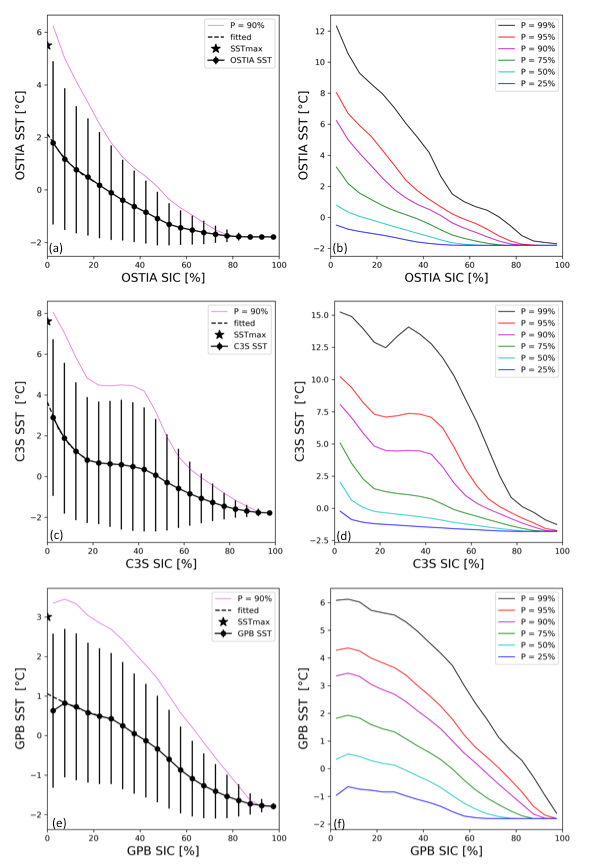
\includegraphics[trim={0 20cm 10.7cm 0}, clip]{EastwoodSST}
    \caption{\label{fig:sst-uncertain}Sea-surface temperature analysis plotted against sea ice concentration. The mean and standard error is computed with 5\% sea ice concentration intervals. The figure is modified from \protect\citet{Castro2023}}
\end{figure}

Figures \ref{fig:leave-one-out}, \ref{fig:noisy} and \ref{fig:swapped} also show that the model gains no skill from the linear sea ice trend computed from the OSI SAF observations. In figure \ref{fig:leave-one-out}, this is shown as model performance is similar with and without the predictor. In figure \ref{fig:swapped} it is seen as the trend follows the baseline and exerts no variability when swapped with trends from other seasons. It can however be seen in figure \ref{fig:noisy} that replacing the trend with uniform noise improves some seasons, although slightly. This may show that the linear trend predictor have a very slight degrading effect on the deep learning forecast, however it can also be model hallucination as the other figures \ref{fig:leave-one-out} or \ref{fig:swapped} does not recreate a similar trend.

\subsubsection{Model inferred physics}
\label{sec:discuss_model_inferred_phys}
The same precautions regarding out-of-distribution samples given in section \ref{sec:discuss_explain} also apply to the synthetic AROME Arctic samples explored in section \ref{sec:synthetic_preds}, since the synthetic fields are likely to contain out-of-distribution combinations of valid values which have not been covered by the training dataset. The purpose of conducting a experiment inspired by sensitivity analysis for physical models is to explore the possibility of applying a similar methodology for diagnosing a deep learning model.

With respect to the forecast errors obtained when comparing a non-synthetic forecast with a forecast where one or several AROME Arctic fields have been replaced with a synthetic variation in figure \ref{fig:synthetic_aa_niiee}, no clear seasonal cycle to the NIIEE can be seen. Such a random change in NIIEE for the same synthetic field at different seasons may show that the model is able to infer some relationship between the state of a physical field and the other predictors. This is further demonstrated by the two synthetic fields in the lower leftmost plot in figure \ref{fig:synthetic_aa_niiee} where the model improved the NIIEE when being fed no-winds or only positive winds in the x direction. Although there is possibility of these results occurring stochastically, it is noteworthy that there may be a possibility to engineer more ideal conditions if the state of other predictors are known.

These results in section \ref{sec:synthetic_preds} also indicate that the model does interpret each atmospheric field separately at the beginning of the encoder before the first convolutional layer merges the different input channels into common feature maps, since the model is able to evolve the sea ice concentration field differently given different states of the atmosphere. Additionally, when figure \ref{fig:synthetic_aa_niiee} is seen in relation to swapping the order of a single AROME Arctic field in figure \ref{fig:swapped}, the general model response to a modified state of the atmosphere is to degrade the forecast skill. This is expected given that the 2-meter temperature and the wind fields are assumed to have a strong correlation, such that when an uncorrelated atmospheric field is introduced to the predictor pool, the encoded signal is weaker resulting in less skillful forecasts.

The response to some of the synthetic AROME Arctic predictions in figure \ref{fig:synthetic_aa_niiee} was shown in figure \ref{fig:synthetic_aa_bias} as spatial biases. The top row of figure \ref{fig:synthetic_aa_bias} shows model response to synthetic wind fields, whereas the bottom row shows model response to synthetic 2-meter temperature fields. A major difference between the top and bottom row of figure \ref{fig:synthetic_aa_bias} is where sea ice growth and decline occur. For the top row, where only the winds are synthetic, it appears that the spatial distribution of sea ice is located where sea ice already exists. However, for the 2-meter temperature synthetic fields in the bottom row, it is seen that the sea ice growth and decline occurs throughout the entirety of the scene, without relation to where the sea ice concentration is located in the recent sea ice chart predictor. This response is compliant with the expected physical interactions between the sea ice and atmosphere. 

Firstly, the x and y-components of the wind are only able to affect sea ice dynamics for already existing sea ice \citep{Spreen2011, Yu2020}. From the upper leftmost plot in figure \ref{fig:synthetic_aa_bias}, it can be seen that when both wind components are negatively oriented, the extent of the sea ice edge is lowered. This is compliant with how the sea ice edge tends to be sharply defined when experiencing incoming winds, since the negative direction of the wind restricts the outward transportation of low concentration sea ice \citep{Yu2020}. The contrary seems to occur in the top right plot in figure \ref{fig:synthetic_aa_bias}, since the sea ice edge is relatively normal to the direction of the winds (only x wind in positive direction) causing the winds to transport sea ice away from the sea ice edge. This is reflected by some areas experiencing a wider MIZ, although with some inconsistencies which may be due to the positive x-wind not affecting the scene in isolation. Secondly, with synthetic 2-meter temperature fields the deep learning system is able to infer growth in areas where there are no sea ice in the recent sea ice chart similar to the occurrence of sea ice formation as a response to freezing temperatures \citep{Hibler1979}. Furthermore, the lower rightmost plot in figure \ref{fig:synthetic_aa_bias} shows a 2-meter temperature field which linearly increases from the lowest possible to the highest possible values in the test data starting in the Atlantic Sea between Norway and Greenland and moving to the Eastern end of the Barents Sea between Frans Josef land and Novaya Semlya as well as the Arctic Sea North of Frans Josef land. The sea ice concentration response to the synthetic forcing is similar, with growth South-East of Svalbard and melt in the parts of the domain East of Svalbard, as expected with regards to the physical response where cold temperatures facilitate sea ice growth and vice versa \citep{Hibler1979}. These results indicate that the deep learning system is able to infer physical relationships and responses from the predictors without having learnt them explicitly. Furthermore, the deep learning system is able to recreate physical responses between predictors to some degree, without having the framework to simulate or resolve the underlying physics.

It is noted that the confidence for the presented synthetic predictions are unknown. Despite the claim in \citet{DeVries2018} regarding that the measurable model confidence may remain high when out-of-distribution samples are utilized, human trust in the deep learning predictions should be lowered proportional to how much out-of-sample the predictors are. E.g. regarding Figure \ref{fig:synthetic_aa_bias}d the 2-meter temperature values close to 235K are far below the modelled minimum 2-meter temperature from ERA5 which is close to 253K over the Atlantic Ocean, but more representative of the minimum 2-meter temperature found above the Central Pack ice (Malte Müller, Pers. Commun.). Furthermore, much of the sea ice growth is occurring in the warm regime of the Arctic ocean south of the polar front \citep{Johannessen1978} in areas in the sea ice charts where sea ice is never present. Hence the synthetic 2-meter temperature field used as input for Figure \ref{fig:synthetic_aa_bias}d does not represent a possible input-output combination in the training or validation datasets. Regardless it is interesting to see that the Deep learning model have some response to the synthetic AROME Arctic fields.

\subsubsection{Explainable predictions}
\label{sec:discuss_seggradcam}
This work opted to implemented the seg-GradCAM technique \citep{Vinogradova2020} to increase the transparency and explainability of the developed deep learning system. An initial attempt implementing the technique for the Deep learning system with a two day lead time at different target contours was shown in figure \ref{fig:seg_base_cont}. The visually highlighted region seems to follow the marked sea ice edge, although the regions in figure \ref{fig:seg_base_cont} (b, c and d) also seems to include parts of Svalbard to a greater extent than (a) showing that the model look at different regions to determine the different contours. Each output layer is attempting to predict is whether the pixels belongs to the cumulative contour represented by the output layer. Figure \ref{fig:seg_base_cont} shows that the regions of the predictors which were important for predicting pixels as part of the cumulative contour were the pixels which constituted the predictor sea ice chart. Although for some contours the model is utilizing pixels outside the sea ice edge, Figure \ref{fig:seg_base_cont} shows that most pixels outside of the sea ice edge is not important for predicting the cumulative contours.

In section \ref{sec:discuss_depth}, is was shown that the 256 depth U-Net without a scene-encompassing theoretical receptive field at the bottleneck outperformed the deeper model where each feature in the bottleneck had a receptive field which covered the bottleneck. It was discussed in Section \ref{sec:discuss_depth} that the effective receptive field covered a fraction of the theoretical receptive field \citep{Luo2017}. Based on figure \ref{fig:seg_base_cont} it can also be seen that by increasing the theoretical receptive field, each encoded feature in the bottleneck are based on a lot of features from unimportant spatial locations. On the contrary, a model such as the 256 U-Net architecture which only had a theoretical receptive field of 145 in the bottleneck would have some features in the bottleneck only computed from important pixels, and some encoded features only computed from unimportant pixels. Thus, it may be the case for the 256 depth U-Net that since some of the feature maps in the bottleneck are based only on important pixels (and vice versa), the signal is easier to decode. Comparatively, when all features are a mix of important and unimportant pixels as for the 1028 depth U-Net architecture, the signal provided by the bottleneck is more difficult to decode. Thus, figure \ref{fig:seg_base_cont} also indicates that it is not necessarily positive for all features in the bottleneck to cover the entire scene, as not all pixels are equally important for predicting the cumulative contours hence diluting the features in the bottleneck with unimportant features.

A comparison is made between the activation maps from the baseline deep learning model in figure \ref{fig:seg_base_cont} and the activation maps from the model with reduced classes in figure \ref{fig:seg_red_cont}. The immediate difference is that the highlighted regions in figure \ref{fig:seg_red_cont} are of much higher importance, compared to figure \ref{fig:seg_base_cont}. However, it is noted that the baseline model has been used to create activation maps for different dates in figure \ref{fig:seg_base_dates} which shows higher importance akin to the values in figure \ref{fig:seg_red_cont}. It is not known if figure \ref{fig:seg_base_cont} contains unusually low values. Despite the general difference in strength between the activation maps in figures \ref{fig:seg_base_cont} and \ref{fig:seg_red_cont}, it is noted that they differ in how they rank land pixels such as Frans Josef Land and Novaya Semlya in terms of importance. In figure \ref{fig:seg_base_cont} pixels related to Frans Josef Land is deemed very important for all contours, and this is also seen in figure \ref{fig:seg_base_dates} (a). It is also seen that Novaya Semlya and Svalbard achieve importance simultaneously starting at figure \ref{fig:seg_base_cont} (b). Although only one date is inspected, this may be related to the shared decoder dicussed in sections \ref{sec:tuning_model} and \ref{sec:performance_confidence}. What figure \ref{fig:seg_red_cont} might demonstrate is that when the fast-ice contour is removed as a target, the previously described negative interactions between the fast-ice contour which is spatially different from the other predicted cumulative contours are not occurring. As a result, the reduced classes model is assigning less importance to the area, compared to the baseline model in figure \ref{fig:seg_base_cont} where Frans Josef Land is assigned high importance as potentially the fast-ice cumulative contour is covering that area only. This might be a consequence of training the baseline model, since the error backpropagated through the network had an additional fast-ice component mainly situated around the land-masses in the scene, causing the model to be tuned towards lowering errors in that area. Consequently, when the baseline model is making predictions, the land-covered pixels are attenuated more since the model has been explicitly fed information of the land pixels through the fast-ice contour. On the other hand, the reduced classes models which have not targeted the fast-ice contour explicitly, have been trained on cumulative contours which resemble each other. In summary, the important pixels may to some degree resemble the shared sea ice contour areas in the cumulative contours, such that when a cumulative contour which offers a significantly limited spatial extent compared to the other contours is used as target, the important regions of the image is reduced to the shared regions between all contours. It is believed that this is a consequence of the shared decoder, due to the previously described negative interactions and effect on the loss each field has.

\subsubsection{decreased skill from 2-meter temperature}
\label{sec:discuss_seggrad_t2m}
It was shown in figure \ref{fig:leave-one-out} that model performance marginally improved when not including 2-meter temperature from AROME Arctic. A repeat run proved that this result was consistent (orange line figure \ref{fig:leave-one-out}). Hence, despite deeming AROME Arctic as a significant contributor to model performance, figure \ref{fig:leave-one-out} indicates that this is due to the two wind components. Despite 2-meter temperature causing model performance to decrease, figure \ref{fig:noisy} and \ref{fig:swapped} show that the model is strongly fitted to the 2-meter temperature, especially during summer and autumn, since both modifications cause model performance to deteriorate. Since AROME Arctic in large is covered by sea ice \citep{Mueller2017}, many of the atmospheric variables are directly affected by the sea ice representation e.g. \citep{Mueller2017, Batrak2018, Batrak2019, Mueller2023}. For 2-meter temperature, a rapid decrease in temperature occurs at the sea ice edge \citep{Mueller2023} (see also figures \ref{fig:case_preds} (a) and \ref{fig:case_atmos} (a)). Thus, it is likely that the deep learning system is able to infer some correlation between the recent ice chart and 2-meter temperature field in terms of defining the predicted sea ice edge. This might explain why the model is strongly fitted towards 2-meter temperature. 

Figure \ref{fig:seg_not2m_dates} showed that the highlighted regions extent beyond the sea ice edge for a model without 2-meter temperature as a predictor, when compared to the baseline model showed in figure \ref{fig:seg_base_dates}. Inspecting figure \ref{fig:seg_not2m_dates} while at the same time considering that the baseline model is potentially strongly fitted to the 2-meter temperature as discussed above, it may be the case that the model without 2-meter temperature is attempting to remedy missing information related to the sea ice edge by looking beyond the sea ice edge. In some scenes, such as figure \ref{fig:seg_not2m_dates} (a) and (b), the model is also considering the land-covered pixels from mainland Norway and Russia as important information, which may be due to the land-sea mask predictor consistently providing the model with a signal covering that area. Furthermore, in autumn (this also occurs to a degree during summer), the model without 2-meter temperature is able to deem pixels related to sea ice in the fjords of Svalbard as important, despite the 2-meter temperature values following the sea ice edge to some extent as seen in figure \ref{fig:t2m_dates}(c). Hence, it seems that the 2-meter temperature predictor implements a spatial inspection barrier determining if the model is using pixels outside the sea ice edge or not. This might occur due to the possible strong correlation inferred by the deep learning system between the recent sea ice chart and 2-meter temperature, such that when the two predictors are working in tangent they amplify the position of the sea ice edge. Consequently, this causes the model to distinguish if each pixel belongs to the MIZ or not, with only pixels inside the inferred MIZ having importance when forecasting a scene. This can have a severe limiting effect on model performance, since information is restricted to pixels only inside the recent sea ice chart.

\subsubsection{Interpreting the case study}
A case study was conducted for the prediction from the test data which achieved the highest NIIEE, with the input, target and prediction presented in figure \ref{fig:case_preds}. Figure \ref{fig:case_preds} (c) demonstrates the smoothing effect of the deep learning prediction as discussed in section \ref{sec:discuss_perf_leadtimes}. However, given the operational use case intended for the forecasts, the smoothness represents variability and to some degree uncertainty which is preferred over more detailed forecasts which are at a higher risk of wrongful predictions. From a user perspective, a generalized view of the sea ice development may prove more valuable than a detailed resolve of certain sea ice structures \citep{Murphy1993}.

In section \ref{sec:discuss_model_response} it was noted that the model was very strongly fitted to the recent ice chart, and as a result the output is expected to resemble an adjusted version of the input. This is shown in figure \ref{fig:case_preds} through two examples. Firstly, notice the red contour directly north of the easternmost part of Frans Josef land in the predictor. In the target, this contour is seemingly cut off, whereas in the deep learning forecast, the contour itself has been deformed rather than removed. The second example are the gradually decreasing contours between Frans Josef Land and Novaya Semlya, which in the target has seen a rapid growth in the red contour nearly covering up all of the orange contour. For the deep learning forecast, the contours from the predictor are mostly preserved albeit smoothened.

Based on the strength of the 2-meter temperature in figure \ref{fig:case_atmos} (a), the temperatures above the sea ice edge seem vary around 273K, which might imply that the scene in figure \ref{fig:case_preds} is mainly wind driven. However, it is not assumed that the deep learning system is interpreting the temperature values, since the convolutional layers derive features from gradients. With respect to the discussion in section \ref{sec:discuss_seggrad_t2m}, the spatial inspection barrier should follow a combination of the sea ice edge in \ref{fig:case_preds} (a) and the temperature gradients which can be inferred visually in figure \ref{fig:case_atmos}.

The atmospheric conditions are shown in figure \ref{fig:case_atmos}. Firstly, southeast of Svalbard there appears to be winds blowing in the positive y-direction, as well as slightly negative with close to 0 m/s x-winds, for where the pixels are assumed to be important (see section \ref{sec:discuss_seggradcam}). Thus the winds are blowing in a direction which appears to be parallel along the sea ice edge, directed towards the Atlantic Ocean with the sea ice edge on the left. Based on the direction of the wind vector, Ekman transport is occurring in the ocean directed away from the sea ice edge (to the right of the wind vector). Consequently, the Ekman transport directed away from the sea ice edge transports sea ice with it \citep{Fennel1998} such that the sea ice edge will expand, and it can be seen in figure \ref{fig:case_preds} (c) that the deep learning system inferred this response for the current example by predicting a wider MIZ in the area. Although the target sea ice chart have moved less, a similar response seems to have happened.

Finally, figure \ref{fig:case_iiee} gives a spatial representation of where the forecast error is located. Based on the IIEE distribution, it is clear that the opening occurring in the sea ice east of Svalbard has a large role in increasing the NIIEE. As there are no indication of a long term bias in the 2-meter temperature field in figure \ref{fig:case_atmos} (a), it is difficult to predict that such a rapid sea ice loss event may happen. It can be seen in AMSR2 passive microwave observations (Supportive Figure \ref{fig:S-amsr2-16} and \ref{fig:S-amsr2-18}) that the sea ice opening North-East of Svalbard had already occurred at the forecast start date, but it was not represented in the sea ice charts before 18th March (Figure \ref{fig:case_preds}b). Moreover, signs of the sea ice opening North-East of Svalbard was already present in the AMSR2 observations at the start of March (not shown). This shows that the sea ice charts are not following all observed events. Given that no maritime operators are expected to (or should) traverse into the opening North-East of Svalbard \citep{Stocker2020}, it is understandable that the sea ice specialist is distributing resources into precisely drawing the MIZ which is of use for maritime end users. However, the discrepancy between the sea ice charts in Figure \ref{fig:case_preds}a,b and Supportive Figures \ref{fig:S-amsr2-16} and {\ref{fig:S-amsr2-18}} shows a potential problem of utilizing manual sea ice charts as a predictor, since subjective artefacts are present in the data. Furthermore, in terms of the model inferred physics and correlation between input predictors it may be problematic if the sea ice concentration is not reflective of the other physical predictor. This is exemplified by the lack of strong 2-meter temperature (Figure \ref{fig:case_atmos}a) located where a large portion of sea ice melted in Figure \ref{fig:case_preds}a,b, which was not occurring since the sea ice had already melted (Figure \ref{fig:S-amsr2-16}).

Given the discussion in section \ref{sec:discuss_model_inferred_phys}, if a warm bias was located above the region it could have prompted the model to decrease the sea ice concentration. Although it might have been shown in the linear sea ice trend, figure \ref{fig:leave-one-out} and \ref{fig:swapped} demonstrated that the trend was not utilized by the model at all, thus it was not considered for the case study. If there was a hole present in the region in the latest sea ice chart predictor, it may be more likely that the model would deform that pattern. Given that the rapid sea ice loss is an unlikely event, which is at most covered by a very limited number of samples and not generalizable, figure \ref{fig:case_preds} demonstrates that spurious sea ice formation / decline events are not well resolved by the deep learning system.

\biblio
\end{document}